\documentclass[11pt]{article}

\usepackage[margin=1in]{geometry}
\usepackage{amsmath}
\usepackage{amssymb}
\usepackage{graphicx}
\usepackage{booktabs}
\usepackage{hyperref}

\title{The correction beyond Zel'dovich is transverse: a measured mechanism for shell-crossing models of cosmic-web transport}
\author{Igor Moiseev}
\date{\normalsize\itshape Draft --- 2026-07-05. Source of every number: the experiment reports in \normalfont\texttt{research/cosmic-web/docs/} \itshape (E0--E12, T1, MODEL-CARD).}

\begin{document}

\maketitle

\begin{abstract}
Lagrangian approximations to cosmic structure formation --- the Zel'dovich approximation (ZA), 2LPT, adhesion, and shell-crossing prescriptions of the MUSCLE class --- are the transport engines of fast mock catalogues and reconstruction, yet \emph{why} shell-crossing corrections outperform perturbative ones has not been directly measured. Using particle-mesh (PM) $N$-body simulations evolved from the same initial conditions as the approximations they test, we measure the residual between true transport and each particle's own ZA prediction in the local tidal eigenframe. The residual is large near the web (RMS $\approx 4.4\,h^{-1}$Mpc within $2\,h^{-1}$Mpc of filament spines) and biased perpendicular to the filament axis at \emph{all} distances ($\langle(\hat{R}\cdot e_3)^2\rangle = 0.21$--$0.30$ versus the isotropic $1/3$; 6 simulations $\times$ 50,000 particles). A single-ingredient model built from exactly this measurement --- ZA rays plus partial ($\beta = 0.6$) transverse momentum damping at first shell-crossing --- reduces held-out median transport error from 4.98 to 4.52 $h^{-1}$Mpc, within 0.05 of the frame-information oracle bound (4.47), and statistically ties MUSCLE ($4.49 \pm 0.12$ vs $4.52 \pm 0.18$, 3 seeds) while 2LPT degrades to 8.07. With frozen parameters the advantage persists across $\sigma_8 \in [0.6, 1.0]$ (growing with clustering, $-3\% \rightarrow -13\%$), voxel scales 0.5--2 $h^{-1}$Mpc, and EdS versus flat $\Lambda$CDM. The exact variational structure of the ZA/adhesion flow --- Hopf--Lax quadratic-cost optimal transport on a flat metric --- identifies the measured term as the shock-formation correction: shell-crossing models work because they implement transverse arrest.
\end{abstract}

\section{Introduction}
\label{sec:intro}

Fast approximations to gravitational transport underpin much of large-scale-structure practice. The Zel'dovich approximation (ZA; \cite{zeldovich1970}) moves mass on straight ballistic trajectories set by the initial gravitational potential; second-order Lagrangian perturbation theory (2LPT; \cite{bouchet1995,scoccimarro1998}) adds the leading nonlinear correction; the adhesion model \cite{gurbatov1989} regularises the ZA's multi-streaming with an infinitesimal Burgers viscosity so that matter sticks at shell-crossing; spherical-collapse remappings and their multiscale extension MUSCLE \cite{neyrinck2013,neyrinck2016} replace the ZA divergence with a collapse-aware prescription; ALPT \cite{kitaura2013} splits scales between 2LPT and spherical collapse; COLA \cite{tassev2013} trades exactness for a few corrective time steps. A consistent empirical pattern runs through this literature: at nonlinear scales, prescriptions that \emph{arrest} particles at shell-crossing beat prescriptions that \emph{perturb} their trajectories --- MUSCLE-class models outperform 2LPT, which is known to overshoot in collapsed regions. What has been missing is a direct measurement of the correction these models are implicitly supplying: the residual between true gravitational transport and the ZA prediction, resolved in the frame that organises collapse.

This paper supplies that measurement and traces its consequences. It is a mechanism paper, not a better-engine paper: the model we build is a probe of \emph{why} shell-crossing corrections work, and its headline result is that a single directional ingredient reproduces MUSCLE-level transport accuracy.

Our contributions, in order:

\begin{enumerate}
\item \textbf{A direct measurement of the beyond-ZA correction (Section~\ref{sec:residual}).} In PM $N$-body simulations evolved from the same initial conditions, the per-particle residual $R = x_{\mathrm{true}} - x_{\mathrm{ZA}}$ is large near the web and preferentially \emph{perpendicular} to the filament axis in the local tidal eigenframe at all distances: $\langle(\hat{R}\cdot e_3)^2\rangle = 0.21$--$0.30$ versus the isotropic $1/3$, with per-axis RMS ratio $R_\parallel/R_\perp = 0.63$--$0.89$ (6 simulations, 50,000 tracked particles each).
\item \textbf{A sufficiency test (Section~\ref{sec:sufficiency}).} A model containing only this ingredient --- ZA rays plus partial transverse momentum damping at first shell-crossing --- reaches held-out median transport error $4.52 \pm 0.18\,h^{-1}$Mpc versus ZA's $4.98 \pm 0.27$, within 0.05 of an oracle bound ($4.47 \pm 0.12$) obtained by giving the model the true final tidal frames. On identical initial conditions it statistically ties MUSCLE ($4.49 \pm 0.12$) while 2LPT degrades to $8.07 \pm 0.39$. This explains the MUSCLE-class advantage: transverse arrest is the correction budget.
\item \textbf{Robustness with frozen parameters (Section~\ref{sec:robustness}).} The advantage transfers without re-calibration across $\sigma_8 = 0.6$--$1.0$ (growing monotonically with clustering), voxel scales 0.5--2 $h^{-1}$Mpc, and EdS versus flat $\Lambda$CDM ($\Omega_m = 0.31$); the PM truth is converged in time (0.008-voxel shift under step doubling); at the field level the model extends the usable $k$-range of ZA with a rescalable large-scale amplitude deficit.
\item \textbf{A theoretical identification (Section~\ref{sec:theory}).} The exact variational principle of the ZA/adhesion flow is the Hopf--Lax formula --- quadratic-cost optimal transport on a \emph{flat} metric \cite{hopf1950,lax1957,brenier1991,frisch2002}. Filaments are shocks of the transport map, and the measured transverse residual is the shock-formation term.
\item \textbf{Secondary results (Section~\ref{sec:secondary}):} an evaluation-methodology lesson (a proxy-matched comparison manufactured a $p \approx 10^{-14}$ false positive), the outcome of a filament-finder comparison including a descriptor that survives on real survey data, and an observational validation of the extracted web against Planck and ACT Compton-$y$ maps.
\end{enumerate}

\section{Methods}
\label{sec:methods}

\subsection{Truth: PM \texorpdfstring{$N$}{N}-body simulations and convergence}
\label{sec:truth}

Truth throughout is a particle-mesh (PM) $N$-body integrator: $128^3$ grid and $128^3$ particles in a periodic box of $L = 128\,h^{-1}$Mpc (1 voxel = 1 $h^{-1}$Mpc), FFT Poisson solver, kick--drift--kick leapfrog with 90 steps from $a = 0.1$ to $a = 1$, Einstein--de Sitter (EdS) expansion in the primary runs and flat $\Lambda$CDM ($\Omega_m = 0.31$) in the transfer test. Initial conditions are Gaussian fields with a BBKS spectrum normalised to $\sigma_8 = 0.8$ (varied in Section~\ref{sec:robustness}), displaced by ZA to $a = 0.1$. Each approximation under test is evolved from the \emph{same} initial field, so residuals are per-particle and exact.

Time convergence of the truth (E10): doubling to 180 steps shifts the median final position by 0.008 voxels --- three orders of magnitude below the effects measured --- and leaves the model-versus-ZA comparison invariant (advantage $-6.8\%$ against both the 90-step and 180-step truths). Grid convergence is covered by the $256^3$ runs of Section~\ref{sec:robustness}. An external cross-check (E12) validates the integrator against a production code: evolved from the CAMELS CV\_0 initial conditions (2LPT, $\Omega_m = 0.3$, $256^3$ particles, 25 $h^{-1}$Mpc box; \cite{villaescusa2021}), our PM reproduces the official $z = 0$ particle positions to a median matched-ID offset of $0.41\,h^{-1}$Mpc against both Arepo and MP-Gadget truths (which agree with each other to $0.029\,h^{-1}$Mpc median --- the code-consensus scale), with field cross-correlation $r = 0.999$, 0.984, 0.937 at $k = 0.35$, 0.66, $1.26\,h\,\mathrm{Mpc}^{-1}$ --- near-perfect agreement over the full range of scales used in this work, degrading only at $k \gtrsim 2\,h\,\mathrm{Mpc}^{-1}$ ($r = 0.837$ at $k = 2.40$) where PM force softening is expected to bite.

\subsection{The residual measurement (E4)}
\label{sec:residual-measurement}

For each tracked particle we compute $R = x_{\mathrm{true}}(a{=}1) - x_{\mathrm{ZA}}(a{=}1)$ and its velocity analogue $R_v$, where $x_{\mathrm{ZA}}$ is the particle's own Zel'dovich prediction from the shared initial conditions. Residual directions are projected onto the local tidal eigenframe ($e_1$, $e_2$, $e_3$ with $\lambda_1 \geq \lambda_2 \geq \lambda_3$; filament axis along $e_3$), and statistics are binned by distance to the filament spine network extracted from the final density field. The direction statistic $\langle(\hat{R}\cdot e_3)^2\rangle$ has isotropic null $1/3$; values above it mean the correction points along filaments, below it across them. Sample: 6 PM simulations, 50,000 tracked particles each; quoted uncertainties are across-seed standard deviations.

A precursor measurement (E2; 4 PM runs, 50,000 particles each, tracked over $a \in [0.5, 1]$) applied the same protocol to deviations of true trajectories from straight chords, independently of any model.

\subsection{The model: ZA rays with transverse damping at first crossing}
\label{sec:model}

The frozen recipe (fixed by the declared optimisation campaign of E5c/E5d and used unchanged in every subsequent experiment):

\begin{itemize}
\item Evolve particles on straight ZA rays in growth-factor steps $\Delta D = 0.05$ ($\approx$18 steps; no Poisson solves beyond cheap density deposits).
\item At each step, deposit the model's own particles to a density grid.
\item The first time a particle's local density exceeds $\rho_c = 5$, remove {\boldmath$\beta = 60\%$} of its velocity components perpendicular to the local filament axis $e_3$ --- the minor eigenvector of the tidal tensor of the model's own density, smoothed at $2\,h^{-1}$Mpc and refreshed every third step. The along-axis component is never touched.
\end{itemize}

The model has three fixed numbers ($\beta$, $\rho_c$, the smoothing scale). Two structural findings from the campaign: partial damping ($\beta < 1$) is required for self-estimated frames to pay --- at $\beta = 1$ the model's own density feedback over-triggers crossings and cancels the frame gain --- and pancake-ordered sequential damping ($e_1$ then $e_2$) underperforms simple both-perpendicular damping at this resolution (E5c).

\subsection{Baselines and the oracle bound}
\label{sec:baselines}

Four baselines are run from identical initial conditions: plain ZA; an isotropic sticking model (the classical adhesion proxy: all velocity components damped at crossing); 2LPT; and MUSCLE \cite{neyrinck2016}. Additionally, an \emph{oracle} variant of our model replaces the self-estimated tidal frames with frames from the true PM final field (E5b). The oracle is not a competitor but an information bound: it prices how much of the remaining error is frame estimation rather than physics.

\subsection{Evaluation protocol}
\label{sec:protocol}

The primary score is the median per-particle distance between the model's $a = 1$ position and the PM-truth position, in voxels (= $h^{-1}$Mpc), overall and binned by distance to the web (spine network of the final field). Seed discipline: $\rho_c$ was calibrated on seed 1 \emph{by optimising the isotropic competitor} (a competitor-favouring choice); configuration selection used seeds \{2, 3\}; every reported validation number comes from held-out seeds (\{4, 5, 6\}, or the 5 held-out seeds of E5), with jackknife-over-seed errors. Field-level scores (Section~\ref{sec:robustness}) are the cross-correlation $r(k)$ (phase fidelity) and transfer function $T(k)$ (amplitude fidelity) against the truth density field.

This protocol is strict because an earlier phase of the programme demonstrated how a plausible protocol can manufacture a discovery. In a filament-finder benchmark (Section~\ref{sec:lesson}), skeleton length --- the quantity that mechanically buys completeness --- was matched on a proxy (hysteresis-mask volume) rather than on the realised skeleton; the resulting $+0.07$ completeness ``win'' carried $p \approx 10^{-14}$ and was entirely an artifact of a 19\% length mismatch. Every comparison in this paper therefore matches, calibrates, or holds out on the score-determining quantity itself: identical initial conditions, identical truth, frozen knobs, held-out seeds, and a competitor-favouring calibration where a choice had to be made.

\section{Results}
\label{sec:results}

\subsection{The correction beyond ZA is transverse in the tidal frame (E4)}
\label{sec:residual}

Table~\ref{tab:residual} gives the direction and amplitude of the residual $R = x_{\mathrm{true}} - x_{\mathrm{ZA}}$ by distance to the web (6 simulations $\times$ 50,000 particles; mean $\pm$ across-seed sd; isotropic null $1/3$).

\begin{table}[htbp]
\centering
\caption{The measured adjustment term (E4): direction and amplitude of the residual $R = x_{\mathrm{true}} - x_{\mathrm{ZA}}$ by distance to the filament spine (6 simulations $\times$ 50,000 particles; mean $\pm$ across-seed standard deviation; isotropic null $1/3$).}
\label{tab:residual}
\small
\begin{tabular}{lcccccc}
\toprule
$d$ to spine (vox) & $n$/seed & $\langle(\hat{R}\cdot e_3)^2\rangle$ & $\langle(\hat{R}_v\cdot e_3)^2\rangle$ & RMS $R_\parallel$ (vox) & RMS $R_\perp$ per axis (vox) & $R_\parallel/R_\perp$ \\
\midrule
0--2   & 20,658 & $0.298 \pm 0.002$ & $0.312 \pm 0.003$ & 4.36 & 4.92 & 0.89 \\
2--4   & 7,269  & $0.297 \pm 0.004$ & $0.300 \pm 0.004$ & 3.77 & 4.19 & 0.90 \\
4--8   & 6,632  & $0.264 \pm 0.004$ & $0.280 \pm 0.003$ & 2.40 & 3.07 & 0.78 \\
8--16  & 10,320 & $0.218 \pm 0.002$ & $0.218 \pm 0.003$ & 1.86 & 2.91 & 0.64 \\
16--64 & 5,120  & $0.208 \pm 0.003$ & $0.203 \pm 0.003$ & 1.77 & 2.83 & 0.63 \\
\bottomrule
\end{tabular}
\end{table}

\begin{figure}[htbp]
\centering
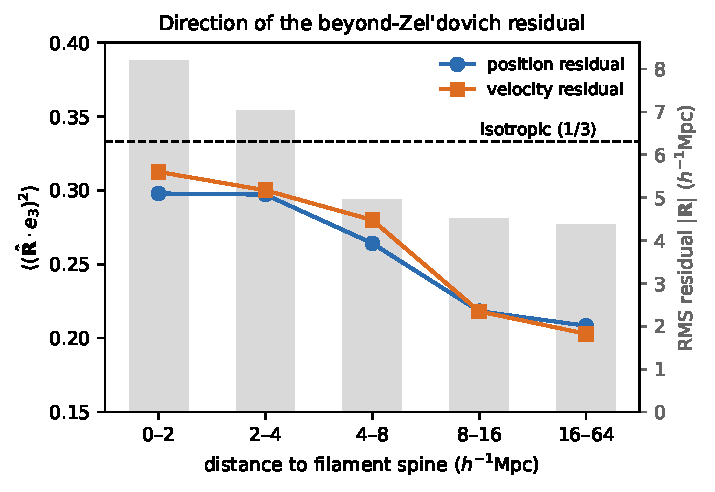
\includegraphics[width=0.75\textwidth]{../docs/paper-figures/fig1_residual_direction.pdf}
\caption{Direction and amplitude of the beyond-ZA residual $R = x_{\mathrm{true}} - x_{\mathrm{ZA}}$ in the local tidal eigenframe, binned by distance to the filament spine (E4; 6 simulations $\times$ 50,000 particles). Lines (left axis): the direction statistic $\langle(\hat{R}\cdot e_3)^2\rangle$ for the position (circles) and velocity (squares) residuals; the dashed line marks the isotropic null $1/3$. Grey bars (right axis): RMS residual amplitude $|R|$ in $h^{-1}$Mpc. The correction is largest near the web (RMS $\approx 4.4\,h^{-1}$Mpc within $2\,h^{-1}$Mpc of spines) and points perpendicular to the filament axis at every distance ($\langle(\hat{R}\cdot e_3)^2\rangle = 0.21$--$0.30 < 1/3$).}
\label{fig:residual}
\end{figure}

Three facts. (i) The correction is large where structure forms: RMS $\approx 4.4$ voxels within 2 voxels of spines. (ii) It is organised by the tidal eigenframe --- the statistics deviate strongly from isotropy. (iii) Its direction is \emph{perpendicular} to the filament axis at every distance: $\langle(\hat{R}\cdot e_3)^2\rangle = 0.21$--$0.30 < 1/3$ and $R_\parallel/R_\perp = 0.63$--$0.89$ everywhere, approaching (but never reaching) isotropy inside the tubes. Physically: ballistic ZA transport overshoots through forming walls and filaments, and the correction real gravity applies is transverse arrest at the web --- not enhanced transport along it.

The model-independent precursor (E2) agrees: deviations of true trajectories from straight chords are perpendicular to the filament axis in the bulk ($\langle(\widehat{\mathrm{dev}}\cdot e_3)^2\rangle = 0.208$--$0.233$ at 8--64 voxels, versus $1/3$), turning weakly parallel ($0.364 \pm 0.010$) only within $\sim$4 voxels of spines, with velocity--axis alignment nearly flat ($\langle|\hat{v}\cdot e_3|\rangle = 0.537$--$0.572$, null 0.5; 4 simulations $\times$ 50,000 particles). Transverse pancake infall --- the Zel'dovich collapse sequence --- is what the instrument recovers, from scratch.

\subsection{One ingredient suffices: the damping model reaches the frame bound and ties MUSCLE (E5--E5d, E9)}
\label{sec:sufficiency}

Table~\ref{tab:ladder} tracks the model from first test to frozen recipe. All entries are median per-particle transport error in voxels against PM truth.

\begin{table}[htbp]
\centering
\caption{The model ladder. All entries are median per-particle transport error in voxels against PM truth.}
\label{tab:ladder}
\small
\begin{tabular}{llccc}
\toprule
stage & configuration & held-out seeds & overall error & vs ZA \\
\midrule
ZA baseline & --- & 5 & $5.00 \pm 0.22$ & --- \\
isotropic sticking (adhesion proxy) & full damping, all directions & 5 & $5.34 \pm 0.15$ & $+7\%$ \\
E5: first transverse model & $\beta = 1$, ZA-proxy frames & 5 & $4.91 \pm 0.14$ & $-2\%$ \\
E5c: refined & $\beta = 0.75$, self-density frames & 3 (seeds 4--6) & $4.64 \pm 0.18$ & $-7\%$ \\
E5d: \textbf{frozen recipe} & $\beta = 0.6$, $2\,h^{-1}$Mpc frames & 3 (seeds 4--6) & {\boldmath$4.52 \pm 0.18$} & {\boldmath$-9\%$} \\
E5b: oracle bound & true final-field frames & 5 & $4.47 \pm 0.12$ & $-10\%$ \\
\bottomrule
\end{tabular}
\end{table}

\begin{figure}[htbp]
\centering
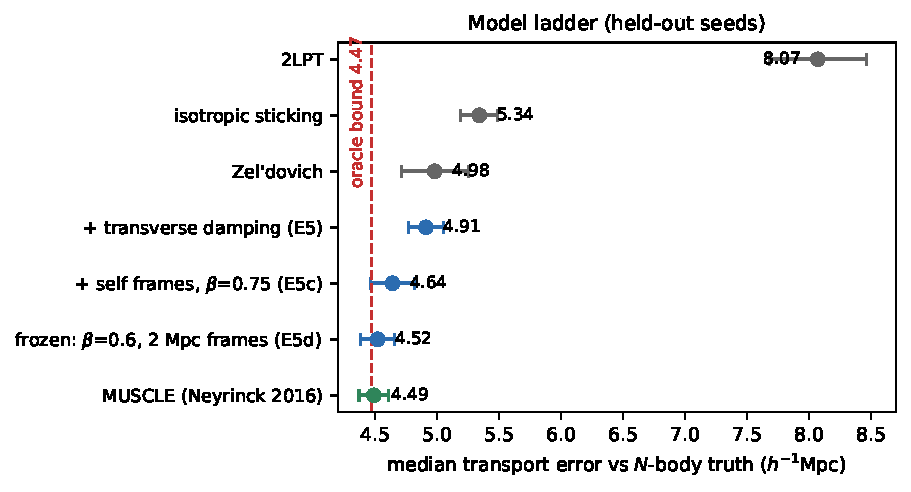
\includegraphics[width=0.85\textwidth]{../docs/paper-figures/fig2_model_ladder.pdf}
\caption{The model ladder on held-out seeds: median per-particle transport error against PM $N$-body truth, in $h^{-1}$Mpc. Adding the single measured ingredient --- transverse momentum damping at first shell-crossing --- carries ZA (4.98) through successive refinements to the frozen recipe ($\beta = 0.6$, $2\,h^{-1}$Mpc self-estimated frames; $4.52 \pm 0.18$), within 0.05 of the oracle bound obtained with true final-field frames (4.47, dashed line) and a statistical tie with MUSCLE \cite{neyrinck2016} ($4.49 \pm 0.12$). Isotropic sticking (5.34) and 2LPT (8.07) degrade transport relative to ZA.}
\label{fig:ladder}
\end{figure}

with the ZA reference at $4.98 \pm 0.27$ on seeds 4--6. The largest gains sit exactly where the correction was measured: at 0--2 voxels from spines the first model already beats ZA by 7\% and isotropic sticking by 14\% ($6.46 \pm 0.07$ vs $6.95 \pm 0.24$ vs $7.50 \pm 0.10$); the oracle shows $-20\%$ available at the web ($5.53 \pm 0.08$). The frozen recipe lands 0.05 voxels above the oracle bound --- 89\% of the recoverable gap closed --- and the oracle experiment (E5b) shows the model beats ZA in \emph{every} distance bin once frames are exact, so the small 2--4-voxel deficit of the practical model ($+4\%$ vs ZA in E5) is frame-estimation error, not wrong physics.

Table~\ref{tab:baselines} places the frozen model against the literature baselines on identical initial conditions (E9; 3 seeds; jackknife errors).

\begin{table}[htbp]
\centering
\caption{Literature baselines, identical initial conditions (E9; 3 seeds; jackknife errors). Entries are median per-particle transport error in voxels against PM truth.}
\label{tab:baselines}
\begin{tabular}{lcc}
\toprule
model & overall error (vox) & web (0--2 vox) error \\
\midrule
ZA & $4.97 \pm 0.27$ & $6.92 \pm 0.31$ \\
2LPT & $8.07 \pm 0.39$ & $8.21 \pm 0.35$ \\
MUSCLE & $4.49 \pm 0.12$ & $5.57 \pm 0.07$ \\
transverse damping (frozen) & $4.52 \pm 0.18$ & $5.77 \pm 0.16$ \\
\bottomrule
\end{tabular}
\end{table}

2LPT \emph{degrades} transport at these nonlinear scales --- the known shell-crossing overshoot. MUSCLE statistically ties the frozen model overall and is slightly ahead at the web; at the field level (Section~\ref{sec:robustness}) MUSCLE wins small-scale phases while the damping model wins mid-scale amplitudes. This is the mechanism result: a model containing \emph{only} the measured ingredient --- transverse arrest at first crossing, in self-estimated tidal frames --- reproduces MUSCLE-class transport accuracy. We conclude that shell-crossing corrections of the MUSCLE class work \emph{because} they implement transverse arrest; the multiscale spherical-collapse machinery is one implementation of a correction whose measured form is directional damping across the web.

\subsection{Robustness: frozen knobs across clustering, resolution, cosmology; field-level fidelity (E6--E8, E10)}
\label{sec:robustness}

Table~\ref{tab:transfer} collects the transfer tests. All use the frozen recipe with no re-calibration; errors in the resolution rows are in physical $h^{-1}$Mpc.

\begin{table}[htbp]
\centering
\caption{Transfer with frozen parameters. All conditions use the frozen recipe with no re-calibration; errors in the resolution rows are in physical $h^{-1}$Mpc.}
\label{tab:transfer}
\small
\begin{tabular}{lccccccc}
\toprule
condition & seeds & ZA overall & model overall & $\Delta$ overall & ZA web & model web & $\Delta$ web \\
\midrule
base (EdS, $\sigma_8 = 0.8$, $1\,h^{-1}$Mpc vox) & 3 & 4.98 & 4.52 & $-9\%$ & 6.93 & 5.78 & $-17\%$ \\
coarse ($2\,h^{-1}$Mpc voxels) & 3 & 2.09 & 2.04 & $-2\%$ & 3.37 & 3.08 & $-9\%$ \\
$\sigma_8 = 0.6$ & 3 & 2.98 & 2.89 & $-3\%$ & 4.73 & 4.26 & $-10\%$ \\
$\sigma_8 = 1.0$ & 3 & 7.20 & 6.23 & $-13\%$ & 9.36 & 7.33 & $-22\%$ \\
flat $\Lambda$CDM, $\Omega_m = 0.31$ & 3 & 4.93 & 4.45 & $-10\%$ & 6.90 & 5.73 & $-17\%$ \\
$0.5\,h^{-1}$Mpc voxels (EdS) & 1 (+2 in E7b) & 4.95 & 4.45 & $-10\%$ & 6.76 & 5.72 & $-15\%$ \\
\bottomrule
\end{tabular}
\end{table}

\begin{figure}[htbp]
\centering
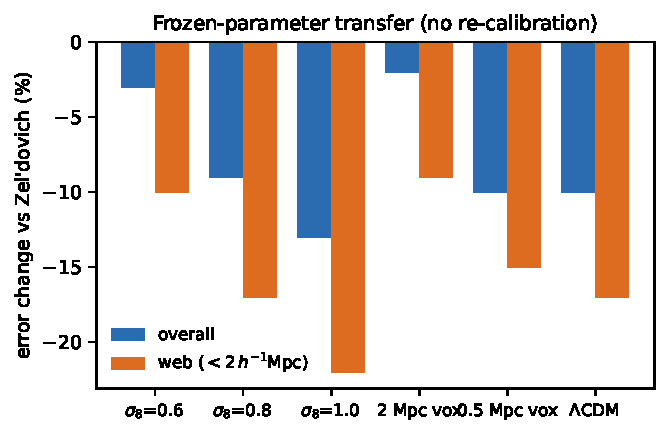
\includegraphics[width=0.75\textwidth]{../docs/paper-figures/fig3_transfer.pdf}
\caption{Frozen-parameter transfer (no re-calibration): change in median transport error relative to ZA, in percent (negative is better), overall (blue) and within $2\,h^{-1}$Mpc of the web (orange). The advantage grows monotonically with clustering amplitude ($-3\% \rightarrow -9\% \rightarrow -13\%$ overall over $\sigma_8 = 0.6$, 0.8, 1.0), persists across voxel scales 0.5--2 $h^{-1}$Mpc, and is unchanged from EdS to flat $\Lambda$CDM ($\Omega_m = 0.31$).}
\label{fig:transfer}
\end{figure}

The advantage grows monotonically with clustering amplitude ($-3\% \rightarrow -9\% \rightarrow -13\%$ overall; $-10\% \rightarrow -17\% \rightarrow -22\%$ at the web over $\sigma_8 = 0.6$, 0.8, 1.0) --- the behaviour expected of a physical shell-crossing correction, since higher $\sigma_8$ means more crossings, not of a tuned artifact. Under $\Lambda$CDM the numbers match EdS almost exactly, as expected for a growth-factor-parametrised geometric term. At $0.5\,h^{-1}$Mpc voxels the physical-unit errors are nearly identical to the $1\,h^{-1}$Mpc runs --- the error scale is set by the physics, not the grid; the two additional seeds of E7b confirm the row at $n = 3$ ($-12\%$ and $-9\%$).

Field-level fidelity (E8; 3 seeds, $1\,h^{-1}$Mpc voxels): the model beats ZA on both cross-correlation and transfer amplitude in the nonlinear regime --- $r(k = 0.53\,h\,\mathrm{Mpc}^{-1}) = 0.388$ vs 0.288, $T(k = 0.34) = 0.410$ vs 0.229 --- extending the usable $k$-range of a ZA-based mock, while the classical isotropic sticking model destroys phase fidelity at all $k > 0.1\,h\,\mathrm{Mpc}^{-1}$ ($r = 0.089$ at $k = 0.53$). Costs, quantified: a $\sim$7\% amplitude deficit in the largest-scale bin ($T = 0.849$ vs ZA's 0.920 at $k = 0.06\,h\,\mathrm{Mpc}^{-1}$), removable by the standard linear transfer rescaling, and a small phase cost at intermediate $k$ ($r = 0.962$ vs 0.975 at $k = 0.14$). Against the baselines (E9): MUSCLE leads $r(k)$ at small scales (0.527 vs 0.388 at $k = 0.53$) while the damping model leads $T(k)$ at mid scales (0.739 vs 0.669 at $k = 0.14$) --- complementary strengths that suggest a hybrid.

\begin{figure}[htbp]
\centering
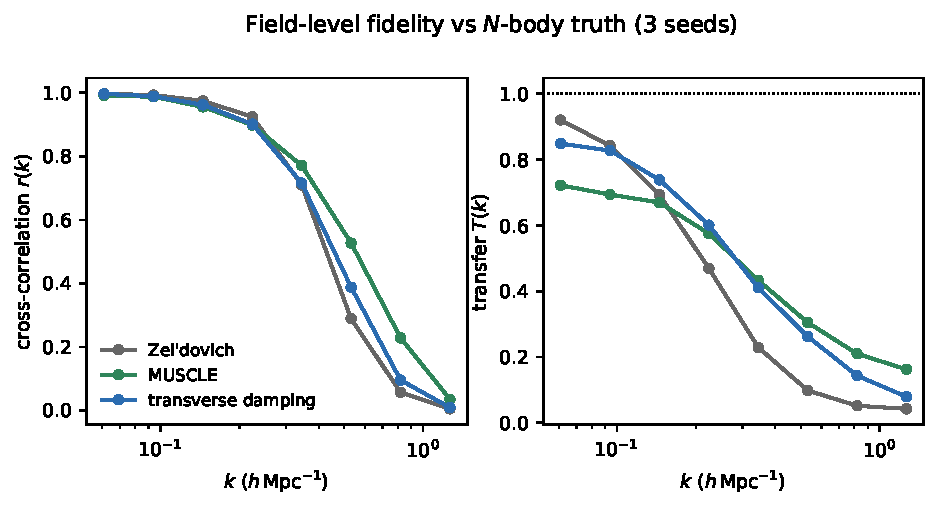
\includegraphics[width=\textwidth]{../docs/paper-figures/fig4_field_level.pdf}
\caption{Field-level fidelity against PM $N$-body truth (E8/E9; 3 seeds, $1\,h^{-1}$Mpc voxels). Left: cross-correlation $r(k)$ (phase fidelity). Right: transfer function $T(k)$ (amplitude fidelity). The transverse-damping model extends the usable $k$-range of ZA ($r = 0.388$ vs 0.288 at $k = 0.53\,h\,\mathrm{Mpc}^{-1}$; $T = 0.410$ vs 0.229 at $k = 0.34$) at the cost of a $\sim$7\% amplitude deficit in the largest-scale bin ($T = 0.849$ vs 0.920 at $k = 0.06$), removable by the standard linear rescaling. MUSCLE leads small-scale phases (0.527 vs 0.388 at $k = 0.53$) while the damping model leads mid-scale amplitudes ($T = 0.739$ vs 0.669 at $k = 0.14$) --- complementary strengths.}
\label{fig:field}
\end{figure}

\section{Theoretical interpretation: shocks of a flat optimal-transport map (T1)}
\label{sec:theory}

The measured transverse correction has an exact home in the variational structure of the models it corrects. Two short steps (full derivation in the programme's theory note, T1):

\textbf{ZA is free motion in growth-factor time.} Writing the Zel'dovich map with the linear growth factor $D$ as time, $x(q, D) = q - D\nabla_q \Phi_0(q)$, every trajectory is a straight line traversed at constant velocity: the potential exerts no force during the evolution --- it is absorbed entirely into the initial velocities. The trajectories extremise the free action $\int |dx/dD|^2\, dD$, i.e.\ they are geodesics of the \emph{flat} Euclidean metric. (This also refutes, constructively, any Jacobi-type ``effective metric'' picture in which paths are cheap along potential valleys: in the variables where the flow is simple there is no potential along the path left to conformalise.)

\textbf{Adhesion is Hopf--Lax, i.e.\ quadratic-cost optimal transport.} The adhesion model regularises multi-streaming with Burgers dynamics $\partial_D v + (v\cdot\nabla)v = \nu\Delta v$, $\nu \to 0^+$, $v = \nabla\psi$. The Hopf--Cole transformation solves it exactly, and the vanishing-viscosity limit is the Hopf--Lax formula $\psi(x, D) = \min_q\, [\psi_0(q) + |x - q|^2/2D]$ --- a minimisation over straight-line transport paths with quadratic cost: precisely the Monge--Kantorovich optimal-transport structure \cite{hopf1950,lax1957,brenier1991}, used cosmologically in the MAK reconstruction \cite{frisch2002,brenier2003}.

The geometry of cosmic-web transport is therefore flat metric, straight rays, plus a Legendre-type convexification of the initial potential. Filaments and nodes are the loci where the Hopf--Lax minimiser jumps between branches --- the \textbf{shock set (caustics) of the transport map} --- not geodesics of any curved or lifted metric. Structure lives in the singularities of the map, not in curved paths.

This derivation predicts the measurements of Section~\ref{sec:residual} before they are made: matter arrives at a filament along straight inertial rays that terminate \emph{on} the shock set --- generically transverse to it (E2/E4: direction statistics below $1/3$ everywhere) --- and after absorption the surviving degree of freedom is the tangential pre-shock velocity, giving weak along-filament streaming inside the tube (E2: $0.364 \pm 0.010$ within $\sim$4 voxels). The correction beyond ZA is, exactly, the shock-formation term: what happens to the transverse momentum at first crossing. Our model implements this term directly ($\beta = 0.6$ rather than the adhesion model's implicit full absorption), and Section~\ref{sec:sufficiency} shows the single term carries the entire measurable correction budget at these scales.

\section{Secondary results}
\label{sec:secondary}

\subsection{The evaluation-methodology lesson: proxy matching and reference circularity}
\label{sec:lesson}

The programme began as a filament-finder comparison and produced its most instructive result there. Comparing skeletons requires matched total spine length, because length mechanically buys completeness. The first benchmark enforced the match on a proxy --- hysteresis-mask volume --- assuming realised skeleton lengths would follow. They did not: the orientation-lift method's skeletons came out $\sim$19\% longer at sparse sampling (1,468 vs 1,239 voxels), and the resulting ``$+0.07$ completeness, 48/50 seeds, $p \approx 10^{-14}$'' advantage was pure length. Under the corrected extractor (iterative correction until the realised skeleton hits the target length) the sign flips: the Hessian baseline wins completeness at every sampling level from 2,500 galaxies up ($\Delta = -0.045$ to $-0.066$ across both curvature variants, the lift winning at most 3/50 seeds, $p \leq 8\times10^{-10}$ everywhere and $\approx 10^{-15}$ at most levels), with a statistical tie only at 1,200 ($\Delta = +0.003/+0.004$, $p = 0.47/0.36$) --- and pushing sparser still (400--600 galaxies) the Hessian wins again ($\Delta = -0.017/-0.021$, $p \approx 0.003$, 30 seeds). The artifact was detected only because a later instrument change retroactively shifted archived scores; the archived length fields confirmed the mismatch. The lesson generalises: \emph{a matched comparison must enforce the match on the quantity that determines the score, and statistical strength ($p \approx 10^{-14}$) does not certify that the comparison was constructed correctly.}

A second protocol failure was caught by design: scoring sparse-data skeletons against a clean-field \emph{reference skeleton} is circular, because each method scores 0.07--0.19 higher against the reference extracted by its own family (E1, $2\times2$ reference matrix, 12 seeds; the two clean references agree only at completeness $\approx 0.60$). The replacement criterion --- mass coverage at matched length, which needs no reference --- is what Sections~\ref{sec:results} and~\ref{sec:finders} use. These two lessons motivated the strict protocol of Section~\ref{sec:protocol}.

\subsection{The filament-finder comparison: single-scale Hessian \texorpdfstring{$\geq$}{>=} SE(3) orientation lift; the anisotropy descriptor survives}
\label{sec:finders}

Under honest matching, the simple single-scale Hessian ridge detector matches or beats the SE(3) orientation-lift detector essentially everywhere tested: exact-truth toys at every density (above), and gravity-shaped fields under the method-neutral mass criterion --- on truncated-ZA boxes at all sampling levels (band coverage $0.2860 \pm 0.0149$ vs the lift's best $0.2691 \pm 0.0139$ at 5,000 galaxies, $p \approx 10^{-3}$, 12 seeds), on PM $N$-body fields (where the shortest-cigar lift closes to a statistical tie at sparse sampling: $\Delta = -0.0045$, $p = 0.55$, 8 seeds), and at $256^3$ resolution (6 seeds). The lift's hypoelliptic-diffusion component is rejected outright: strong diffusion is harmful at every curvature and sparsity tested ($-0.06$ to $-0.12$, $p \approx 2\times10^{-6}$), weak diffusion buys $+0.01$ ($p = 0.03$) only at ultra-sparse sampling, and an 8-step Trotter splitting at equal total diffusion reproduces the coarse result --- the verdict is operator-level, not numerical (E0b, E0d). A hybrid summing the two percentile-normalised scores earns a niche: $+0.05$ purity and $+0.040$ junction F1 over the Hessian at 5,000 galaxies ($p = 1.3\times10^{-4}$, 20 seeds) at a $-0.02$ completeness cost (E0c).

What survives for the lifted geometry is a \emph{descriptor} role, consistent with Section~\ref{sec:theory}'s reading (the orientation manifold describes the shock set, not the transport): unweighted lift spines align with the clean-field tidal eigenvector $e_3$ at 0.734--0.759 versus the Hessian's 0.665--0.674 (isotropic null 0.5; E1, 12 seeds), and this replicates on the real Universe --- $0.677 \pm 0.016$ vs $0.617 \pm 0.016$ across 18 independent BOSS CMASS tiles (E3). The lifted skeleton reads the anisotropy of the web better even where it loses on mass.

\subsection{Observational validation: the extracted web sits on real gas}
\label{sec:observational}

The web that the pipeline extracts from data is physically real. Stacking spine networks from 274,075 BOSS CMASS-North galaxies ($z = 0.45$--$0.55$, 18 tiles of $512\,h^{-1}$Mpc at $4\,h^{-1}$Mpc voxels) on the Planck Compton-$y$ map yields an excess of $8.99\sigma$ (Hessian spines; $6.86\sigma$ lift) against 200 null sets matched to the spine points' galactic-latitude histogram --- stricter controls \emph{strengthened} the first-pass $4.8\sigma$/$4.1\sigma$ detection (E3, E3b; 41,535/40,426 spine points). Masking the tracer halos ($7'$) leaves $1.95\sigma$/$0.07\sigma$: the spine-stack signal is dominantly the tracers' own halo gas, and an ACT DR6 test of the masked residual at arcminute resolution stayed below the pre-registered $3\sigma$ gate ($1.77\sigma$ at $3'$, $1.11\sigma$ at $7'$; E3c).

The between-halo component was instead measured with a pair-bridge estimator: $y$ at the midpoint of close CMASS pairs (876,639 pairs, transverse separation 6--14 $h^{-1}$Mpc, line-of-sight $< 6\,h^{-1}$Mpc) minus ring controls at $\pm 60^\circ/\pm 90^\circ/\pm 120^\circ$, which cancels any circularly symmetric halo by construction (E3d-v2). Under the full validity battery (E3e) --- jackknife errors over 50 RA patches (pair bootstrap is optimistic by 1.6--2.4$\times$) and physically unconnected null pairs (same transverse window, line-of-sight 25--40 $h^{-1}$Mpc) --- the on-axis excess is $3.30\sigma$ on ACT and $7.99\sigma$ on Planck, the null pairs expose a $4.7\sigma$ beam-leakage term on Planck ($1.80\times10^{-8}$) and none on ACT ($1.65\sigma$), and the null-subtracted bridge amplitude is $1.4\times10^{-8} \pm 0.9$ ($\approx 1.6\sigma$, ACT) and $1.2\times10^{-8} \pm 0.5$ ($\approx 2.2\sigma$, Planck) --- mutually consistent and matching published LRG-pair bridge amplitudes ($\sim$1--2$\times10^{-8}$; \cite{degraaff2019,tanimura2019}). We report this as a reproduction of the literature amplitude with honest errors and physical nulls at $\sim$2$\sigma$ per instrument, not as an independent detection.

\section{Limitations}
\label{sec:limitations}

\begin{itemize}
\item \textbf{PM-only truth, externally checked at one configuration.} All transport truths come from our own particle-mesh integrator: time-converged (0.008-voxel shift under step doubling, E10), grid-checked at $256^3$, and validated against Arepo on the CAMELS CV\_0 box (median matched-ID offset $0.41\,h^{-1}$Mpc; $r \geq 0.93$ for $k \leq 1.3\,h\,\mathrm{Mpc}^{-1}$, E12). Residual caveat: the external check covers one box size and cosmology; PM force softening still suppresses small-scale amplitudes ($T \approx 0.86$--$0.92$ at the checked scales), a bias partially shared between truth and models.
\item \textbf{EdS-primary.} The primary calibration and most experiments use Einstein--de Sitter expansion; $\Lambda$CDM is verified at one configuration ($\Omega_m = 0.31$, 3 seeds) with matching numbers, consistent with a growth-factor-parametrised term, but no broader cosmology scan was run.
\item \textbf{One-shot damping.} The model damps at \emph{first} shell-crossing only; multi-stream interiors are out of scope by design. The residual error at the web (5.5--6 voxels even at the oracle bound) is post-crossing physics that no first-crossing rule can represent; do not interpret model positions within $\sim$2 voxels of density peaks as resolved halo structure.
\item \textbf{BBKS spectrum.} Initial conditions use the BBKS transfer function rather than a Boltzmann-code spectrum; the mechanism measurement should be insensitive to this, but absolute numbers may shift.
\item \textbf{Seed counts.} Held-out validation uses 3--5 seeds per condition (single seed for the first $0.5\,h^{-1}$Mpc row, extended to 3); errors are jackknife-over-seed. The consistency of the advantage across every condition mitigates, but does not replace, larger ensembles.
\item \textbf{Calibration locality.} $\beta$ and $\rho_c$ were calibrated at this box size and tracer density; the transfer tests hold them frozen successfully across the scoped ranges ($\sigma_8$ 0.6--1.0, voxels 0.5--2 $h^{-1}$Mpc, EdS/$\Lambda$CDM), but new regimes warrant re-calibration against a small PM truth, optimising the competitor first.
\item \textbf{Large-scale amplitude.} The field-level deficit at the largest scales ($\sim$7\% in $T(k)$ at $k = 0.06\,h\,\mathrm{Mpc}^{-1}$) requires the standard linear rescaling before use in mocks.
\end{itemize}

\section{Conclusions}
\label{sec:conclusions}

We measured the correction that ballistic (Zel'dovich) transport needs in order to match $N$-body gravity, resolved in the frame that organises gravitational collapse. The measurement is unambiguous: the correction is large near the web and points across the filament axis at every distance --- transverse arrest, not enhanced along-filament transport. A model containing only that ingredient --- straight ZA rays plus 60\% transverse momentum damping at first shell-crossing in self-estimated tidal frames --- closes 89\% of the gap to its own frame-information bound, ties the best shell-crossing prescription in the literature (MUSCLE) on transport, beats the classical isotropic adhesion proxy everywhere, and transfers with frozen parameters across clustering amplitude, resolution, and cosmology, with the advantage growing where crossings multiply. The theory closes the loop: the exact variational structure of ZA/adhesion is flat quadratic-cost optimal transport, filaments are the shocks of that map, and the measured term is the shock-formation correction.

The practical conclusion for the fast-mock literature is a mechanism, not an engine: MUSCLE-class shell-crossing corrections work because they implement transverse arrest. The two model families' complementary field-level strengths --- MUSCLE's small-scale phases, transverse damping's mid-scale amplitudes --- suggest a hybrid as the natural next engine, but not a naive one: triggering the directional damping on MUSCLE's precomputed Lagrangian collapse times underperforms both parents ($4.67 \pm 0.18$ vs 4.49/4.52, weakest at the web; E11), so the evolving Eulerian density carries trigger information the Lagrangian collapse time lacks, and MUSCLE's own advantage must live in its displacement-divergence construction rather than its trigger. Hybridisation therefore has to happen at the displacement/field level; the natural next measurement is the second-crossing term that both model families currently omit.

\section*{Data availability}

All code, per-experiment reports with full tables and $p$-values, per-seed result files, and one-command reproduction scripts are in the repository under \texttt{research/cosmic-web/} (experiments E0--E12 and T1: \texttt{docs/}; runners: \texttt{scripts/}; per-seed numbers: \texttt{artifacts/}), including the model card with the frozen recipe and integration guide (\texttt{docs/MODEL-CARD.md}): \url{https://github.com/moiseevigor/moiseevigor.github.io/tree/research/geometry-of-cosmic-web/research/cosmic-web}

\begin{thebibliography}{99}

\bibitem{aragon2007} Arag\'{o}n-Calvo, M. A., et al. (2007). ``The multiscale morphology filter: identifying and extracting spatial patterns in the galaxy distribution.'' \emph{A\&A} 474, 315--338.

\bibitem{bond1996} Bond, J. R., Kofman, L., \& Pogosyan, D. (1996). ``How filaments of galaxies are woven into the cosmic web.'' \emph{Nature} 380, 603--606.

\bibitem{bouchet1995} Bouchet, F. R., Colombi, S., Hivon, E., \& Juszkiewicz, R. (1995). ``Perturbative Lagrangian approach to gravitational instability.'' \emph{A\&A} 296, 575.

\bibitem{brenier1991} Brenier, Y. (1991). ``Polar factorization and monotone rearrangement of vector-valued functions.'' \emph{Comm. Pure Appl. Math.} 44, 375--417.

\bibitem{brenier2003} Brenier, Y., Frisch, U., et al. (2003). ``Reconstruction of the early Universe as a convex optimization problem.'' \emph{MNRAS} 346, 501--524.

\bibitem{cautun2013} Cautun, M., van de Weygaert, R., \& Jones, B. J. T. (2013). ``NEXUS: tracing the cosmic web connection.'' \emph{MNRAS} 429, 1286--1308.

\bibitem{codis2012} Codis, S., et al. (2012). ``Connecting the cosmic web to the spin of dark haloes.'' \emph{MNRAS} 427, 3320--3336.

\bibitem{degraaff2019} de Graaff, A., et al. (2019). ``Probing the missing baryons with the Sunyaev--Zel'dovich effect from filaments.'' \emph{A\&A} 624, A48.

\bibitem{duits2011} Duits, R., \& Franken, E. (2011). ``Left-invariant diffusions on the space of positions and orientations and their application to crossing-preserving smoothing of HARDI images.'' \emph{Int. J. Comput. Vis.} 92, 231--264.

\bibitem{duits2014} Duits, R., Boscain, U., Rossi, F., \& Sachkov, Yu. (2014). ``Association fields via cuspless sub-Riemannian geodesics in SE(2).'' \emph{J. Math. Imaging Vis.} 49, 384--417.

\bibitem{epps2017} Epps, S. D., \& Hudson, M. J. (2017). ``The weak-lensing masses of filaments between luminous red galaxies.'' \emph{MNRAS} 468, 2605--2613.

\bibitem{frisch2002} Frisch, U., Matarrese, S., Mohayaee, R., \& Sobolevski, A. (2002). ``A reconstruction of the initial conditions of the Universe by optimal mass transportation.'' \emph{Nature} 417, 260--262.

\bibitem{gurbatov1989} Gurbatov, S. N., Saichev, A. I., \& Shandarin, S. F. (1989). ``The large-scale structure of the universe in the frame of the model equation of non-linear diffusion.'' \emph{MNRAS} 236, 385--402.

\bibitem{hahn2007} Hahn, O., Porciani, C., Carollo, C. M., \& Dekel, A. (2007). ``Properties of dark matter haloes in clusters, filaments, sheets and voids.'' \emph{MNRAS} 375, 489--499.

\bibitem{hopf1950} Hopf, E. (1950). ``The partial differential equation $u_t + u u_x = \mu u_{xx}$.'' \emph{Comm. Pure Appl. Math.} 3, 201--230.

\bibitem{kitaura2013} Kitaura, F.-S., \& He\ss{}, S. (2013). ``Cosmological structure formation with augmented Lagrangian perturbation theory.'' \emph{MNRAS} (Letters).

\bibitem{lax1957} Lax, P. D. (1957). ``Hyperbolic systems of conservation laws II.'' \emph{Comm. Pure Appl. Math.} 10, 537--566.

\bibitem{libeskind2018} Libeskind, N. I., et al. (2018). ``Tracing the cosmic web.'' \emph{MNRAS} 473, 1195--1217.

\bibitem{neyrinck2013} Neyrinck, M. C. (2013). ``Quantifying distortions of the Lagrangian dark-matter mesh in cosmology.'' \emph{MNRAS}.

\bibitem{neyrinck2016} Neyrinck, M. C. (2016). ``Truthing the stretch: non-perturbative cosmological realizations with multiscale spherical collapse (MUSCLE).'' \emph{MNRAS}.

\bibitem{portegies2015} Portegies, J., Sanguinetti, G., Meesters, S., \& Duits, R. (2015). ``New approximation of a scale space kernel on SE(3) and applications in neuroimaging.'' \emph{SSVM 2015}, LNCS 9087.

\bibitem{scoccimarro1998} Scoccimarro, R. (1998). ``Transients from initial conditions: a perturbative analysis.'' \emph{MNRAS} 299, 1097--1118.

\bibitem{sousbie2011} Sousbie, T. (2011). ``The persistent structure of the Universe --- I. Theory and implementation.'' \emph{MNRAS} 414, 350--383.

\bibitem{tanimura2019} Tanimura, H., et al. (2019). ``A search for warm/hot gas filaments between pairs of SDSS luminous red galaxies.'' \emph{MNRAS} 483, 223--234.

\bibitem{tassev2013} Tassev, S., Zaldarriaga, M., \& Eisenstein, D. J. (2013). ``Solving large scale structure in ten easy steps with COLA.'' \emph{JCAP}.

\bibitem{villaescusa2021} Villaescusa-Navarro, F., et al. (2021). ``The CAMELS project.'' \emph{ApJ} 915, 71.

\bibitem{villaescusa2020} Villaescusa-Navarro, F., et al. (2020). ``The Quijote simulations.'' \emph{ApJS} 250, 2.

\bibitem{zeldovich1970} Zel'dovich, Ya. B. (1970). ``Gravitational instability: an approximate theory for large density perturbations.'' \emph{A\&A} 5, 84--89.

\end{thebibliography}

\end{document}
